%% $RCSfile: proj_report_outline.tex,v $
%% $Revision: 1.3 $
%% $Date: 2016/06/10 03:41:54 $
%% $Author: kevin $

\documentclass[11pt
              , a4paper
             , twoside
              , openright
              ]{report}


\usepackage{float} % lets you have non-floating floats

\usepackage{url} % for typesetting urls

\usepackage{pdfpages} % for adding pdf

\usepackage{graphicx} % for adding graphics

\usepackage{appendix} % for using appendix

\usepackage{url}



%
%  We don't want figures to float so we define
%
\newfloat{fig}{thp}{lof}[chapter]
\floatname{fig}{Figure}

%% These are standard LaTeX definitions for the document
%%                            
\title{Why Do Programmers Do What They Do? \protect\\ A Theory of Influences on Security Practices}
\author{Lavanya Sajwan}

%% This file can be used for creating a wide range of reports
%%  across various Schools
%%
%% Set up some things, mostly for the front page, for your specific document
%
% Current options are:
% [ecs|msor|sms]          Which school you are in.
%                         (msor option retained for reproducing old data)
% [bschonscomp|mcompsci]  Which degree you are doing
%                          You can also specify any other degree by name
%                          (see below)
% [font|image]            Use a font or an image for the VUW logo
%                          The font option will only work on ECS systems
%
\usepackage[image,ecs]{vuwproject}

% You should specifiy your supervisor here with
%     \supervisor{Firstname Lastname}
% use \supervisors if there is more than one supervisor
\supervisors{James Noble, Craig Anslow}

% Unless you've used the bschonscomp or mcompsci
%  options above use
%   \otherdegree{OTHER DEGREE OR DIPLOMA NAME}
% here to specify degree
\otherdegree{Bachelor of Engineering with Honours in Software Engineering}

% Comment this out if you want the date printed.
\date{}

\begin{document}

% Make the page numbering roman, until after the contents, etc.
\frontmatter

%%%%%%%%%%%%%%%%%%%%%%%%%%%%%%%%%%%%%%%%%%%%%%%%%%%%%%%

%%%%%%%%%%%%%%%%%%%%%%%%%%%%%%%%%%%%%%%%%%%%%%%%%%%%%%%

\begin{abstract}

Technologies are continually adapting to match ever-changing trends. As this occurs, new vulnerabilities are exploited by malignant attackers and can cause significant economic damage to companies. Programmers must continually expand their knowledge and skills to protect software. Programmers make mistakes, and this is why we must interpret how they implement and adopt security practices. Understanding these decisions can help inform design and education around improving programming language security.

\end{abstract}

%%%%%%%%%%%%%%%%%%%%%%%%%%%%%%%%%%%%%%%%%%%%%%%%%%%%%%%

\maketitle

\chapter*{Acknowledgements}\label{C:Acknowledge}

I want to thank my supervisors James Noble and Craig Anslow, for their ongoing support and direction as I have completed this project.
\newline
\newline
To dad and mum, thanks for harassing friends to potentially participate in this study. To dad, mum and Saumya, thank you all for having no idea about what I have been doing all year long, but for also leaving me relatively alone for these last weeks as I write, write, write and write. 
\newline
\newline
And to Janaye; a massive thanks for reading over this report and being my grammar and punctuation whizz since high school.

\tableofcontents

% we want a list of the figures we defined
\listof{fig}{Figures}

%%%%%%%%%%%%%%%%%%%%%%%%%%%%%%%%%%%%%%%%%%%%%%%%%%%%%%%

\mainmatter

%%%%%%%%%%%%%%%%%%%%%%%%%%%%%%%%%%%%%%%%%%%%%%%%%%%%%%%

% individual chapters included here
\chapter{Introduction}\label{C:intro}

\par As software is now ubiquitous across industry and it is impossible not to have a presence in the tech sphere. Consequently, software security has become so significant, programmers have to ensure that the security processes that they implement are resilient to any attacks. Lack of attack prevention can cause leakage of sensitive information, massive economic damage and danger to massive numbers of users and employees, consequently opening business, clients and end-users to exploitation by external bodies. Unfortunately, every day, we hear of organisations that have been compromised \cite{1}. Last year New Zealand experienced a significant security breach within the Tū Ora Compass Health (Tū Ora) Primary Health Organisation (PHO) \cite{incident}. Tū Ora is one of the largest PHO's in the country and it governs the greater Wellington region \cite{incident}. Personal information of up to one million New Zealander's was exposed and the effects of this are ongoing \cite{incident}. Ccosts have been great in attempts to mitigate any effects to the public. Dedicated call centres have had to be organised as well as dedicated mental health lines \cite{healthpol, incident}. Regular updates have had to be released in order to maintain communication transparency and assurance quality measures are ongoing \cite{healthpol, incident}.  
\newline
\par Qualitative research is often neglected and overlooked in favour of more quantitative reasoning and technical traits such as the security method used or the programmers task-completion rate \cite{3}. Programmers provide a human aspect to a technical solution and therefore, there should be a shift towards understanding the more background ‘soft’ processes that occur when making decisions; why are the choices made based on past influences, and how they affect the programmers work in the present? 
\newline
\par Past the research aspect, when security and privacy issues do occur in real-world scenarios, developers are blamed first as it is their projects that have allowed the vulnerabilities to be exploited \cite{4}. While developers do make mistakes, they also do need the support to make better security decisions, and this support is currently lacking in the industry \cite{4}. Education is limited past initial acceptance within organisations, and often developers have a blasé attitude to the matter expecting another team to fix the issue \cite{5}. Furthermore, security mechanisms often have an increased complexity, which make them difficult to understand and to then use \cite{6}.
\newline
\par This project will investigate how software developers implement and adopt security practices in the work they do in order to develop an understanding of what influences and impact decisions surrounding their technical work. This project will be conducted using grounded theory which is a theory is a method which aims to establish a theory when there is none \cite{2}, and it is a commonly used method for data analysis. Interviews will take place to collect the data, from which the answers will be analysed to draw conclusions on standard security practices in the professional workplace. This project builds upon works by Hala Assal, Charles Weir and Nathan Newton \cite{summary1, 1, nathan}. 
\newline
\par This project aims to implement a theory as to why programmers implement and adopt security practices in the work they do by interviewing professional developers and using the Grounded Theory Method to analyse the outcomes. Grounded theory is a research method to analyse qualitative data. There are several thorough steps which include; sampling, data collection, data analysis, theoretical note writing, identifying core categories, forming theoretical outlines and presenting a theory.
\newline
\par Participants will be recruited by posting on tech-related groups (i.e. From OWASP Meetup Group and LinkedIn) and mailing lists and also using mine and my supervisor contacts. At this point, I can then start semi-structured interviews with 10-20 interested individuals on their security practices while programming. These people will all be developers in New Zealand that are in varying stages of their careers and career paths to allow for a broader range of responses and a case study relevant to New Zealand. Examples of appropriate job titles include; DevOps engineer, front-end security developer, database administrator, developer, programmer and security architect.
\newline
\par This project will lead to a new, more in-depth understanding of the psychology of the decisions made by programmers. The research done by this project could lead to future qualitative research to be done on another under-developed topic on why programmers do what they do. Paired with this research, that future one could help build a profile of a programmer and their thought processes. Data collected could also be the foundation that allows a developer to build tools that helps other developers implement proper security practices; a Grammarly for security. It can also help the further development of existing static analysis tools such as Infer developed by Facebook, Tricorder used by Google, Coverity and Raygun \cite{infer, tri, coverity, raygun}. These tools all work by providing security detection modules and are used for quality assurance and security. 
\newline
\par Exploring this topic is essential as it allows for a more comprehensive understanding of how and why programmers think the way they do, and of the human and social aspects of Software Engineering \cite{geeks}. We want to understand what solutions developers are using to implement in their security practices, if at all. The findings from this can support developers in terms of education and the better design of security methods in programming \cite{summary1} that have an emphasis on usability. The findings of this project can also be used to identify what security methods developers find as beneficial in their programming. This will allow programmers to complete their work to a high standard, by adhering to proper security protocols, thus overall making their work of a higher value both in a secure and professional sense.

\section{Deviations from the Original Plan}
There have been no deviations from the original plan.
\chapter{Background}\label{C:Background}

\par Conceptually, this project aims to gather data in order to ultimately form a theory. Therefore, It is essential that I know enough information about the topic of security so that I am able to interview professional engineers in a manner which is knowledgeable. This chapter will include background on the importance of information security practices, what practices are widely used, and summaries on existing research on similar subject matter. 

\chapter{Methodology}\label{C:Methodology}

This chapter outlines the methodology that was followed to obtain findings in this study. The methodology is then further deconstructed to describe the data collection and data analysis process. The data collection subsection provides a summary of the participants.

\section{Grounded Theory} 

Grounded Theory (GT) is the chosen methodology for this study. This was an appropriate choice as the study focuses on human aspects, and GT is a way of analysing qualitative data with the end-goal of defining a new theory from the sampled data \cite{geeks}. There are several steps in the GT  methodology in order to make the final theory.  The theory is expected to be explanatory, focusing on describing elements of the findings rather than stating. The theory should also be based on the collected responses and observations, rather than pre-conceived ideas. As such, extensive literature reviews should be avoided.
\newline
\par Initially, researchers must choose a topic and determine whether the Grounded Theory method is the right one for the research project \cite{geeks}. After contacting potential participants, an iterative process of data collection occurs. Questions adapt between the rounds of the collection as the data is analysed. This refinement of questions happens to delve deeper into the traits of the emerging theory. When saturation is achieved, no further new findings are displayed which contribute to the final theory. This results in the “grounded” nature of the overall theory.
\newline
\par 
In the study outlined in this report, at approximately ten interviews, the concepts obtained from the data collection started to become quite similar. This is called saturation point and is when some new lower-level ideas are being obtained, but no overly new information. This was the grounding point of this specific Grounded Theory. 
\newline

\begin{figure}[ht]
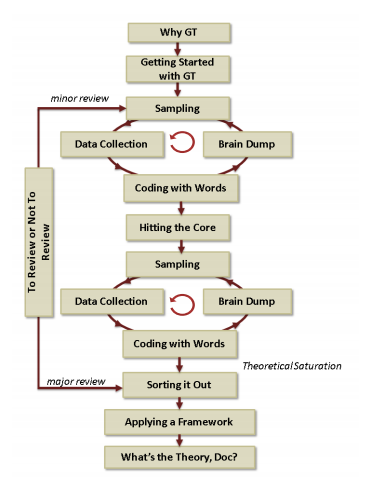
\includegraphics[width=8cm]{figures/fig1.png}
\centering
\caption{The Grounded Theory Pattern (Hoda, Noble, \& Marshall, 2011) Used with Permission \cite{geeks}}
\centering
\end{figure}

\par Initially, I aimed to get more technical empirical evidence on programmers and their security practices. I, however, identified as early as the third interview that technical security programming practices are not as influential as initially thought, and the interview questions changed to match this gradual shift in focus. This is another benefit of Grounded Theory as questions do not have to stay the same; instead, they undergo iterations of development as an area of interest shifts.  


\section{Data Collection} 

\subsection{Recruitment}
\par A recruitment post and webpage was sent to mailing lists and websites like OWASP Meetup and LinkedIn \cite{webpage}. These are shown in Appendix E and Appendix F, respectively. There was a brief halt in the recruiting through the Meetup website as I got banned for posting in groups as I was marked as spam. However, I did not get much interest from the promotion through both Meetup and Linkedin and instead relied on personal contacts (friends and family-friends) and supervisor contacts for initial recruitment. Participants also helped with recruitment by reaching out to others in the industry and telling them about this study. 

\subsection{Interviews}

\par Fifteen interviews were conducted with participants across New Zealand. These participants were from fourteen unique organisations. Participants had varying job titles, years of experience, and were in a range of different sectors and organisation fields. The diversity within the participants allowed for connections to be made across a broader range of people. 
\newline
\par Human Ethics approval had to be gained before the interview process could commence (Appendix B). Initial questions were developed based on a small pilot study run on two recent graduates of the School of Engineering at Victoria University of Wellington. Overall, this small pilot study was essential in providing some more clarity on the interview process. It also supplied practice in conducting interviews and has helped in the continuous process of defining questions.
\newline
\par After Human Ethics had been approved the interview process started. Questions were adapted dependent on the analysis between the interviews and changed as a result of participants answers within the interview. This was so any intriguing information could be queried further during the semi-structured interview. Therefore, the list of interview questions in Appendix D changed with only the "Participant Background" section remaining as a constant.
\newline
\par Due to the disruptive year, interviews were predominantly conducted over Zoom. Consent from the participants was obtained through an email response as per Human Ethics committee request. Interviews ran for periods ranging between 30-90 minutes. A summary of the participant sample is provided in the table below. 
\newline
\newline

\begin{table}[!hb]
\begin{tabular}{|l|l|l|}
\hline
\multicolumn{1}{|c|}{\textbf{Alias}} & \multicolumn{1}{|c|}{\textbf{Role}}                           & \multicolumn{1}{|c|}{\textbf{Experience (Years)}} \\ \hline
\multicolumn{1}{|l|}{P1}           & \multicolumn{1}{l|}{Enterprise Architect and Domain Lead}   & \multicolumn{1}{l|}{15\textless{}}             \\ \hline
\multicolumn{1}{|l|}{P2}           & \multicolumn{1}{l|}{Principal Product Architect}            & \multicolumn{1}{l|}{15\textless{}}             \\ \hline
\multicolumn{1}{|l|}{P3}           & \multicolumn{1}{l|}{Senior Security Architect}              & \multicolumn{1}{l|}{10-15}                      \\ \hline
\multicolumn{1}{|l|}{P4}           & \multicolumn{1}{l|}{Senior Software Engineer}               & \multicolumn{1}{l|}{15\textless{}}              \\ \hline
\multicolumn{1}{|l|}{P5}           & \multicolumn{1}{l|}{Software Developer}                     & \multicolumn{1}{l|}{\textless 2}                \\ \hline
\multicolumn{1}{|l|}{P6}           & \multicolumn{1}{l|}{Level 2 Security Analyst}               & \multicolumn{1}{l|}{2-5}                        \\ \hline
\multicolumn{1}{|l|}{P7}           & \multicolumn{1}{l|}{Site Reliability Engineer}              & \multicolumn{1}{l|}{\textless 2}                \\ \hline
\multicolumn{1}{|l|}{P8}           & \multicolumn{1}{l|}{DevOps Engineer}                        & \multicolumn{1}{l|}{\textless 2}                \\ \hline
\multicolumn{1}{|l|}{P9}           & \multicolumn{1}{l|}{Portfolio Architect}                    & \multicolumn{1}{l|}{10-15}                      \\ \hline
\multicolumn{1}{|l|}{P10}          & \multicolumn{1}{l|}{Full-stack Software Developer}          & \multicolumn{1}{l|}{2-5}                        \\ \hline
\multicolumn{1}{|l|}{P11}          & \multicolumn{1}{l|}{Cloud Engineer}                         & \multicolumn{1}{l|}{2-5}                        \\ \hline
\multicolumn{1}{|l|}{P12}          & \multicolumn{1}{l|}{Consultant (Cloud Engineering)}         & \multicolumn{1}{l|}{2-5}                        \\ \hline
\multicolumn{1}{|l|}{P13}          & \multicolumn{1}{l|}{Development Manager and Technical Lead} & \multicolumn{1}{l|}{10-15}                      \\ \hline
\multicolumn{1}{|l|}{P14}          & \multicolumn{1}{l|}{Senior Software Engineer}               & \multicolumn{1}{l|}{10-15}                      \\ \hline
P15                                & Business Rule Consultant                                    & 15\textless{}                                   \\ \hline
\end{tabular}
\centering
\caption{Participant Aliases and Summary}
\centering
\end{table}

\section{Data Analysis} 

After transcribing interviews and pairing them with written observations), the selective coding process occurs \cite{geeks}. Key points from each transcript are paired with a simplified summary of the points \cite{geeks}. The constant comparison method is used where codes are compared to others from within the same interview and also with other interviews \cite{geeks}. These comparisons continue to occur, and are further narrowed to become categories for the theory \cite{geeks}, also referred to as selective coding \cite{geeks}. Therefore, this coding process has three key steps. Theoretical notes are written throughout this coding process to research relationships between concepts and categories \cite{geeks}. An emergent theory is then formed which aims to explain a practice or a phenomenon. 









\chapter{A Theory of Influences on Security Practices}\label{C:Emergent Theory}

This chapter will outline the emergent theory. \textbf{The three-step coding process }s described in the methodology section was used to achieve this theory. The three found categories and the relationship between each of them will be further explained.

\subsection{Emergent Theory}

The emergent theory consists of three main categories on what influence programmers:

\begin{enumerate}
\item  Culture in groups of individuals
\item Organisational structure and practices
\item Industry trends
\end{enumerate}

\begin{figure}[ht]
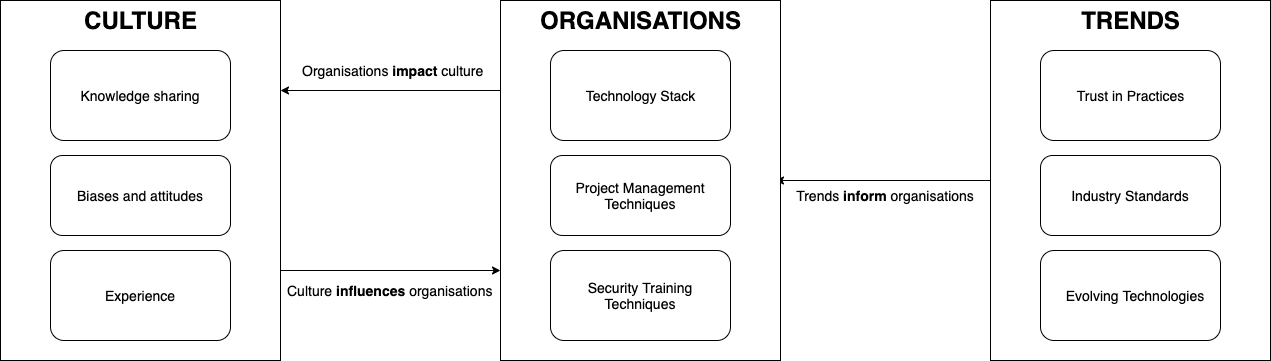
\includegraphics[width=17cm]{figures/fig2.png}
\centering
\caption{The Theory of Influences on Security Practices}
\centering
\end{figure}

\section{Culture}

This category is the effect of the culture we see in groups of individuals. The term culture refers to the customs that programmers have in order to maintain security: knowledge sharing, biases and attitudes and experience. 

\subsection{Knowledge Sharing}

Knowledge sharing is deliberate exchange of information and it was highly regarded among the participants \cite{know}. Participants identified communication between team-mates as being a key way to learn and better current and new security practices. These opportunities are taken within teams and are often done when peer-programming or simply asking questions. 
\newline
\par
\textit{"I like that people come to me when they need help. I think that is the best way for everyone to learn, even me!" - P3}
\newline
\par
Often vital knowledge sharing moments happened in passing. When programmers were stuck with using a library, framework or even learning a newer language nuance, they appreciated the ability to turn to the person next to them and get help. 
\newline
\par \textit{"...we've got a really flat structure, if I needed to I could pretty much directly ping someone..." - P10 }
\newline
\par
Participant \textit{[P8]} defined that the open communication streams between people across business and experiences made it easier to obtain answers. Walking between desks to other teams and also sending anyone emails regardless of hierarchy helped facilitate these exchanges. These exchanges were often more attainable in smaller organisations where individuals were more familiar \textit{{P5, P8, P9}}. 
\newline
\par 
\textit{"It's a lot easier when there are only seven people in my company. - P8"}
\newline
\par
This is harder to maintain in larger organisations. 
\newline
\par
\textit{"You don't do technical inductions which is quite irritating  because you do have to know people and you do have to  find people who know stuff - P11"}
\newline
\par
\textit{"I think bigger companies have very secure processes, and it's very need-to-know and there is a very clear divide and no one is afraid to say that it's above your clearance. Smaller companies the lines are a little bit blurred on clearance... I think [at] the size of that is find because there is communication... I think security is far more approachable in a smaller company; it seems far more reasonable and accessible." - P8}

\subsection{Biases and attitudes}

\par Participants had very strong preferences to how security practices aligned with their work. Those who were strictly developers \textit{[P4, P5, P7]} typically found it a deterrence to completing their work on time, while the others had more of a positive attitude towards managing security. 
\newline
\par 
\textit{"I believe that tasks kind of [get] pushed back a month or two purely because security teams get quite busy on an ad-hoc basis and hiding something, removing something, [adding something], can understandably be a bigger thing, even if it is one manager asking for access... Now we are aware of the leak times that those kind of security tasks can take and so we do plan for those, but I'll also probably say a lot of those times we don't plan enough" - P7}
\newline
\par
\textit{"... It is going to take time, my point was we can manage it nicely without confusing people" - P1}
\newline
\par
This also showed that often, people had a more positive demeanour when dealing with technologies based on familiarity. 
\newline
\par \textit{"... when a change happens that they don't like, there have been people who have straight up left and quit their jobs... their empire is DESTROYED!"  - P11}
\newline
\par
\textit{"For me, I know that it is important so I'm willing to compromise on that on a personal level, but I can get where that someone that it is not their, not their thing, they can see it as a hindrance"  - P12}
\newline
\par One participant \textit{[P11]} acknowledged the personal relationships within the workplace as contributing to biases in the \textit{"tech bro-culture" }. They gave the example of a vendor-client relationship that they had witnessed where the vendor accepted any requests into production because of the close friendship with the client. The client had not given any comments and had caused the build pipeline to fail many times and it was still was not working as the vendor continued to approve changes. This \textit{"tech bro-culture"} also exhibits explicit favouritism between small groups of people in an organisation. People also have a view where asking questions makes you seem lesser than, and therefore, there was a cultivated culture on this lack-of-communication. They stated that a lot of the time in this industry people would say that they know something when they do not. 

\subsection{Experience}

\par Experience pertains to the level of expertise an individual has in the industry. This was not only measured by the amount of years that they have worked, but also whether they have worked on a range of projects. One participant \textit{[P11]} is an example of this; have only worked 2-5 years in industry, but have worked in multiple government and private organisations during this time. They regularly advise the seniors in their team on the work that they do as their experiences are related to their background in the industry.
\newline
\par
\textit{"... Which is a strange dynamic because they're both seniors... Yeah, I'm a lot younger, I'm the only woman and I have a lot more experience than they do in the specific stuff that we're working in right now. And a lot of where my skill-set comes in is like picking up things up quickly because I have moved around a lot, I have done a whole bunch of random stuff".}
\newline
\par
Almost all the participants identified major differences in how less experienced and more experienced individuals deal with security practices. Often less experienced team members are wanting and willing to learn, but still are lacking in the ability to identify key threats and risks which a more experienced team member is more versed in doing. 
\newline
\par
\textit{"New team members, I find, that they're kinda charged-up, ready-to-go, and that they want to prove themselves. I do find the more experienced people are a little more humble and they're a little bit more set-back... it's a bit more of a  different energy-vibe; you see the new people come in, so ready to learn and they want to do security and then you get the people who have been there for ages like oh yeah that's easy and just do it." - P6 }
\newline
\par
\textit{"I am relatively new to the industry so I come in with a fresh mind. " -P5}

\section{Organisations}

This category presents the influence of organisational practices and structuring of security practices. The attributes within this category are the parts of an organisation which motivated programmer choices: technology stack, project management techniques and security training techniques. 

\subsection{Technology Stack}

\par The technology stack is the security tools, frameworks, libraries and languages in use in an organisation. Throughout the study it was prevalent that organisations have existing security programming languages that they use. 
\newline
\par
\textit{"I'd say company-wide [language]... Java for the back-end using spring as the framework and JavaScript for the front-end using React as the framework." - P5}
\newline
\par
\textit{"We go with C\# and React JavaScript because those are the languages more-or-less used around the company" - P7}
\newline
\par
\textit{"We are a Microsoft technology stack company so we are very much on C\#, and so Microsoft C\#, and [the] legacy system has Visual, VB.net" - P13}
\newline
\par
These are chosen based on legacy technologies already in use [P13] and legacy products that organisations provide clients [P3, P7].  Not a lot flexibility is given to programmers to choose language and if they try lobby a change there is a very long term process in approving \textit{[P10]} which dissuade them in trying to make any changes to the current process.
\newline
\par 
\textit{"If you make a request, you don't know when you're going to hear back, so that's one of the constraints... you can prioritise stuff and they can probably get it done, but for other stuff, like I'm trying to get a tool approved... I filled in a form in literally April, and security hasn't gotten back to me. It's kind of an example that security ignores you and you can't use a tool without approval." - P10}
\newline
\par
\textit{"If you ask questions a lot of the time your work gets halted... I don't know what they are doing because they certainly aren't listening to you or replying to your emails." - P11}
\newline
\par
When asked about whether languages changed dependent on security practices and/or requirements the answer was often,
\newline
\par \textit{"No." - P4}.
\newline
\par 
\textit{"I'd say security is not the biggest factor is choosing [a language]" - P7 }
\newline
\par
\textit{"I don't think it is the direct result of security, it's the result of functionality" - P8}
\newline
\par One participant did mention that their libraries and tools did not change based on the security needs as they use ones that can be used across languages [P13].
\newline
\par
\textit{"We haven't seen a library which is not compatible over many languages ... " - P13}
\newline
\par Two outliers that were able to change languages related to security. Both the cloud engineers \textit{[P11, P12]} stated that languages were changed based on their security needs; not on features or familiarity. Especially when working on the security of pipelines, but pipelines themselves were mandated by the organisation. 
\newline
\par
\textit{"...we picked this tool... we also couldn't pick our pipelining tool, that was Jenkins and that's a corporate mandate... I think what makes us different is that we deal with CI/CD so need to keep up-to-date and research more..." - P11}

\subsection{Project Management Techniques}

\par Project management techniques are set by the organisational structuring and choices of more senior people within companies. Participants indicated these project management techniques as effecting how they implemented security in their work. The three project management techniques mentioned in this section are Waterfall, Agile and DevOps. Waterfall is where a development team follows a linear movement in completing a project and any obstructions are not planned for \cite{water} . Agile methodology uses the idea of sprints to define breaking up the original brief into mini-goals \cite{water}. DevOps is the newest trend where instead of delivering a small output at the end of each sprint, there is continuous delivery \cite{ubiq}. Agile and DevOps can both use the idea of cross-functional teams to promote collaboration. 
\newline
\par 
One participant \textit{[P10]} used the Waterfall methodology, while other participants \textit{[P3, P4, P5, P7, P8, P11, P12, P13, P15]} worked with either Agile or DevOps project management. When managed correctly, the techniques benefited participants a lot. It was easier getting the security teams involved throughout the process in a more DevOps approach, and with an Agile approach each deliverable are checked at the end of each sprint, but strict management styles were not enforced. 
\newline
\par
\textit{"It is a major problem with the Waterfall type projects.... it's slowly going out, but very slowly, and they've left a lot of things behind, or rather forgotten to update a bunch of processes to match this stuff... Most places that I've worked, we do Agile, we do DevOps, but [also] not really. It's a whole thing." - P11}
\newline
\par
Traditional waterfall-type management leaks through and some participants felt as though there is an emphasis of security at the beginning and end of projects rather than throughout as a means to reduce \textit{"tech-debt" [P7]} which does the opposite as programmers then struggle to fix multiple issues at the end. 
\newline
\par 
\textit{"I think that it takes the load of developers so developers can just focus on building [a] good application. I think the set-up right now [by having a separate security team] is pretty good right now. I, I just say that it is just annoying putting the request through and them being slow" - P10}
\newline
\par 
Participants with more senior roles \textit{[P3, P4]} did not like the wave of DevOps management; it was identified as being too time consuming or just a fad. The feelings to do with security were different as one was a developer \textit{[P4]} and one was a security architect \textit{[P3]}. The latter critique also stemmed from a hatred of buzz-words when they mentioned DevSecOps; a more security specific iteration of DevOps project management.
\newline
\par \textit{"It's just annoying and gets in the way of my work" - P4}
\newline
\par \textit{"... I don't like it. No one actually follows anything anyway, and an ongoing security approach should be there already..." - P3}
\newline
\par 
The project management techniques also influenced how teams interacted with each other. With a DevOps approach, the support from the security team was continuous and talking between teams occurred more often. . Often a security person was fully involved in the entire project; consequently this increased collaboration meant that security issues were being identified earlier, not just near deadlines or after completion. 
\newline
\par 
\textit{"The cross-functional teams, is how I've kind of been told to refer to them; they're really good... Anyway the point was, yeah, a lot of it is around your organisational structure and the way you form your teams. It's a major problem with like waterfall-type projects where you do like dev, and then you do test and then you do security at the end, but that's, it's slowly going out, but I mean like very slowly, and they've left a lot of things behind, or rather forgotten to update a bunch of processes to match this sort of stuff." - P11}
\newline
\par
This does not often occur due to a lack of resources such as skilled employees and money as different business units charge for time \textit{[P12]}. 
\newline
\par
\textit{"Ideally that [would] be awesome, but you have to pay all those people." - P12 }

\subsection{Security Training Techniques}
\par 
Security training techniques and methods are chosen internally by the organisations. Participants \textit{[P1, P2, P3, P6, P7, P9, P10, P11, P12, P13, P14, P15]} state that they have not been exposed to much security training during their prior education so the training's that work provide are key in educating employers in how to protect assets and mitigate risks and are ongoing. 
\newline
\par 
\textit{"I don't have any formal education, but I have worked in security roles in two other organisations" - P2}
\newline
\par
\textit{"The closest thing really is [learning about] concurrency [at uni] for the most part." - P5}
\newline
\par
\textit{"I had one security paper when I was studying" - P6}
\newline
\par
\textit{"No there were no security specific papers, if anything, it might be a handful of lectures at uni" - P7}
\newline
\par
Training methods are still quite traditional. They are more policy and protocol related and often employees just have to do readings, watch videos or listen to talks in the office by either internal teams or external businesses. The training techniques are more informative to-do's of what to watch out for rather than learning any practical mitigation techniques. 
\newline
\par
\textit{"There was some basic training done for certification... watching stupid videos like Kevin Mitnick" - P4}
\newline
\par 
Organisations do not expect employees to know the policies and protocols, but are expected to know the technical programming-side or should pick them up themselves.
\newline
\par 
\textit{"It's kind of expected, we don't do any formal coding security training, we've got other general security training about data and procedures, but nothing like technical related... I've done, I've had some, listened to some talks throughout about general security risks. They talk about you know, the different areas that our company gets kind of attacked. More, of just of a FYI." - P7}
\newline
\par 
\textit{"People assume that if you're coming into these roles you kind of understand this stuff. But I've seen it go so wrong." - P11}
\newline
\par
Personal training where employees can can search for non-work organised security training sessions. This is encouraged in organisations and a budget is put aside for employees. Participants stated that they could ask to do their own training at work using Linkedin videos or Pluralsight \textit{[P10, P11, P12, P13]}. 
\newline
\par
\textit{"We get given a budget to go pick out what kind of training we want to do." - P6}
\newline
\par 
While the subject of the solo-learning videos are more technically focused, they are still theory-based. This is why most participants identified that they learn best from talking to other people in their teams as you learn more technical skills when you apply your knowledge. 
\newline
\par
\textit{"I'm actually really lucky I work with some great guys. I got paired up with another guy and we sat through and scheduled out six weeks." - P6}
\newline
\par
\textit{"I just ask and someone will help me out and they'll teach me" - P10}
\newline
\par
\textit{"I think the best training you can get is from your peers..." - P14 }
\newline
\par
There were two unique points brought up by participants from my sample group which shows a gradual change in how organisations aim to educate programmers on security. Participant \textit{P10} recalled the use of technical workshops with an external company being a great way to learn how to program more securely to protect applications. This method was a more active approach than what had been described by others. They stated it was similar to following live-coding during university lectures. 
\newline
\par
\textit{"I think at work actually, they also made us do a workshop on SQL injection attacks and stuff and they made us do a bunch of things and we actually had to follow along on our own computers and that's really the only way you learn is by doing." - P10}
\newline
\par 
Another newer way of learning  was corporate Hackathons. These are events which the organisation runs for its employees. Two participants \textit{[P13, P14]} talked highly about it as being fun and casual while also prompting people to learn concepts. 
\newline
\par
\textit{"You can't enforce it... when you do that you that you've lost people. Hackathons are optional and part of [good] culture". - P14}
\newline
\par
The Hackathon topics would be centred around the organisation field (eg. Fintech) in order to translate learning's from these sessions to their current work. 
\newline
\par
\textit{"We have our own in-house, we call it Hackathon, you know, programme and base-line programme where anybody [can join], it's a kind of mandatory training programme where everybody [will go through] - [they] will be given a kind of a training or walk through by one of our security team, team member[s] actually, to how it works, how does it work in reality... People will be given some level of platform information, that what [does] this Hackathon [mean] and it's a game, you know, game! Where can you show me where is [the] problem. Can you fix [the] problem? [Do] you think there is a problem here? Do you think [with this] given website, will you be able to hack some data from my, from the machine, you know? So it's all kind of doing, rather than just doing, a PPT programme, a presentation, [it's] more getting your hands dirty and getting things done. " - P13 }
\newline
\par
\textit{"[I'm] fortunate enough to work in a company where there is a Hackathon every month somewhere in the world right. And, and it's amazing" - P14}

\section{Trends}

\par This category is the influence of industry trends on a programmer. The attributes within this category impact the security related decisions which programmers make: trust in practices, industry standard, evolving technologies. 

\subsection{Trust in Practices}

\par Those who worked in financial tech and in consultancy firms \textit{[P3, P6, P7, P9, P11, P12, P13]} favoured enterprise tools and libraries. These tools provided them with more security in protecting their assets. There are two categories of tools which are enterprise and open-source. Enterprise solutions are paid licenses that provide ongoing support, while open-source are free and built by a community. This can mean that open-source products do not provide long-term support. 
\newline
\par
Those participants did acknowledge that while enterprise was favoured over open-source due to more trust, there were times where open-source was needed when coming across a new problems without any enterprise solution \textit{[P12]}. The participants also used open-source when they wanted to adapt anything to best suit their practices without breaching any legal agreements with the enterprise solutions. 
\newline
\par
\textit{"We do prefer enterprise, but to avoid breaking any SLA's [service level agreements] sometimes we have to look towards other open-source alternatives. We don't prefer it, but have to do it." - P12}
\newline
\par
Every participant stated that while the security team has to vet new software, they do not check libraries. This in turn gives programmers free reign over choice. While the majority did not check the open-source libraries  \textit{[P1, P2, P3, P4, P5, P7, P8, P9, P10, P11, P12, P13, P5]} and one participant \textit{[P10]} stated that all that gets checked is the functionality of the library after it has already been used. Therefore, there is a trust in libraries being secure to use within a applications, but as open-source libraries are built by a community of people, there is no surety. 
\newline
\par
\textit{"I honestly, like, I don't know, like, I'm really allowed to like code, and use the library and play around with it. - P10"}
\newline
\par
\textit{"It's this really strange thing that I've seen a few times now around in places. They provisionally accept a lot of different pieces of open-source technology which is kind of scary because it's just based on someone vouching for this piece of software." - P11}
\newline
\par
Only one participant who checked open-source libraries before using them \textit{[ P14]}. They stated that open-source libraries are great to use because they have so many different people working on them at once, but it was naive not to check them for any discrepancies or issues, especially since so many are readily available which can make the choosing process overwhelming. This checking defines programmers and their ethics and a lack-of doing this can provide entry-ways to threats.
\newline
\par
\textit{".... there are a certain giveaways which you can look in  the code-base and footprints to actually see if the tools are leaning towards the good-side or bad-side... there are a few giveaways like the test coverage of a tool, linting in the tool. How many commits do you actually do? Do you write any footprint doc for it? How do you add a feature? Is it commented? Types, annotations." - P14}
\newline
\par 
The participants in government organisations or within smaller start-ups had to outsource a lot of the security work \textit{[P1, P5, P8, P9, P15]}. Organisations do not have the resources to dedicate the time into this aspect of programming and consequently, they also do not robustly test any outputs of the vendors against security, only the functionality. 
\newline
\par 
\textit{"I think it's mostly a resource limitation because we don't have that many developers... Yeah that's a no from me." - P5}
\newline
\par
Participants stated have a trusting relationship with their vendors. This relationship was acknowledged that this was not the best practice as a participant [P11] noted that vendors and client both lie so it was better to ask as many questions as possible. 
\newline
\par 
\textit{"There is a lot of like - I'm not quite sure what the right word would be, but basically they try and front very differently. Like if you're a vendor you try and act like you're very, very component and understand everything and are a pro of what you do because that's what you're getting paid for right? But you may not understand everything and because that conversation won't be had that you're like "oh I don't quite understand what the ramifications of not doing that", they will often lie to the client. I've been in meetings where people have blatantly lied. Like vendors have blatantly lied about their experience, how their piece of technology works and like it happens and it's very hard to control it especially when the other-side of the table, often the client who you're dealing with as like a consultant isn't often very technical. So you'll try to explain something to them and they do not understand it, they don't get it, they don't get it past like you're talking some version numbers and you're talking some technology words and they don't get it. So if you can break it down further and further for them, they will sometimes get it, but often they pretend that they understand and will just kind of put a stamp and move on or business will say budget and say no".}
\newline
\par
Another participant stated that a breach due to a vendor designed product was the catalyst for change within their organisation for hiring an internal software team \textit{[P10]}.
\newline
\par
\textit{"Around the time we started doing everything in-house." - P10}

\subsection{Industry Standards}

\par Much of the processes of how programmers worked with security was defined by industry standards. There is a rush to match others in the same field, and also to work inside the legal and best-practice compliance standards. 
\newline
\par 
Participants cited SOC reports and ISO \cite{iso} compliance \textit{[P2, P3, P4, P6, P7]} as being the key frameworks that were followed when coding. ISO is a standard that has requirements (clauses) that organisations need to conform to. SOC has some more adaptability where an organisation is able to meet the criteria in any way. Ultimately, they build trust and are mandates so that programs can be used externally by clients and other parties. 
\newline
\par
\textit{"It's so it can be used by clients or it's not allowed." - P3}
\newline
\par
The clauses and criteria enforce clear coding practices upon programmers such as encryption of their work and separation between applications, \textit{"zero-trust architecture" [P1]}. Programmers also follow the best-practices outlined by OWASP (section 2.3). This does not only include the actual code, but also documentation. 
\newline
\par
\textit{"With the various compliance regimes that we're under, so there's ISO27001, PCI and some stuff for the government we have to demonstrate that we are following the processes." - P2}
\newline
\par
There is a pressure to keep on par with other similar people and companies in industry. This is to still stay relevant in the area of expertise and especially for vendor firms to look appealing for their clients. 
\newline
\par
\textit{"We haven't [stuck] ourselves in any particular way. Whatever industry is responding [to] and whatever the new features and challenges are coming, we adopt it; we adopt as early as possible." P13}

\subsection{Evolving Technologies}

Participants emphasised the emergent and evolving technologies in industry as being a motivator in adapting security practices. Cloud products was one that was consistently bought up in the interviews, and the first participant [P1] stated that in following interviews, I should focus on cloud in order to match the newer ways of working rather than just the old. This emergence of the cloud involves server migration to services like AWS and Azure or data migration. AWS and Azure are prevalent in industry as they are the two cloud services approved my government.  The migration has been slower in New Zealand compared to the rest of the world due to data legally having to be stored on-shore. 
\newline
\par
\textit{"Any organisation private or public, they are putting extra [effort] and going out of the box to [move] onto cloud, and the cloud is totally different compared to the on-prem, legacy infrastructure. - P1"}
\newline
\par 
More resources are also being directed into automation of services \textit{[P15]}. While it costs in terms of time and money in the present, much like server and data migration, there are many long-term savings. 
\newline
\par
These evolving technologies mean that newer processes have to be learnt on how to deal with security. However, this is difficult as not a lot of people have the robust knowledge to truly understand these yet, especially within a client and vendor relationship. 
\newline
\par
\textit{"... a lot of people at the start didn't necessarily know [understand], it wasn't intentional. Sometimes it's also clients, they just go on and add these rules..." -P12}

\section{Relationships between Categories}

\par This section describes the relationships between each of the categories: trends inform organisations, organisations impact culture and then vice versa with culture influencing organisations. 

\subsection{Trends Inform Organisations}

Emergent trends in industry heavily informed organisational practices. This relationship is shown when newer technologies (4.3.3) and standards are released (4.3.2), as there is a rush for organisations to pick up the traits in order to seem relevant, up-to-date and/or within the bounds of the law. This rush is all based on the organisations decisions, and the informed nature means trends just exhibit and provide opportunities for organisations to make any changes. 
\newline
\par When new technologies become popular in industry, organisations adopt them in their technology stack, as seen in the rise of React into the in-use languages \textit{[P3, P5, P7, P10, P13]}. 
\newline
\par 
\textit{"Nowadays React is getting more popular, you know? We as a company have to grow as well and we can't [be] sitting on our past legacy code... We have to offer and we have to adapt those new, we call it as futuristic technology... It has a capacity to adapt new security principles - measures... We see a long lasting future rather than continuing with our legacy process. In terms of productivity, it is more convenient, it is more user-friendly, it is more responsive, it is more secure compared to our legacy. We can't avoid it... We have to keep progressing " - P13 }
\newline
\par
They can also become mandated by the organisation as with Jenkins for the pipeline \textit{[P11]} (4.1.3). The choice of that is because of an industry standard, not explicitly stated by compliance standards or by legislation, but the desire to match and be on-par with other companies.
\newline
\par 
Project management techniques are informed by industry trends as well. The phasing out of traditional Waterfall is due to the emergence of Agile, and now the adoption of DevOps and consequently DevSecOps is another trend. These changes to match the trends seem to be premature and confusing for programmers and how they deal with security as these management styles are not exactly used as how they were designed to be. 
\newline
\par
\textit{"DevSecOps is a new thing that's getting popular in Wellington." - P3}
\newline
\par
There is more of a shift and understanding that there needs to be more technical programming support provided in workplaces with some budget put aside for this by companies (4.2.3). There is not a not strong trend yet, but as established companies \textit{[P10, P2, P14]} continue to do live-coding workshops and internal Hackathons, this will further inform other organisations of the benefits of such security training techniques (4.2.3). 

\subsection{Organisations Impact Culture}

\par Organisations impact the culture of employees within industry. The ways of working in an organisation impact the three aspects of culture: knowledge sharing, biases and attitudes and experience.
\newline
\par
Organisational structure impacts the ability to share knowledge. This is most clearly effected by the project management techniques in use. With a more DevOps approach, there is talking going on throughout the project life-cycle which involves different teams. This is similarly identified in the Agile management styles as best practice is pulling in security team members to assess at the end of each sprint. Participants identified these two methodologies as being extremely helpful. 
\newline
\par
\textit{"I love DevOps, and what it kind of means to me is that we have these cross-functional teams and we make it that you're not throwing over a dead cat to Ops... " - P11}
\newline
\par
These two approaches as opposed to Waterfall also promote communication within teams as the constant assessing makes internal teams discuss whether their solutions are best-practice and they share ways of changing. 
\newline
\par 
\textit{"It's much easier to scale it back rather than catch it, what is it called? DevSecOps." - P12}
\newline
\par
Biases and attitudes are impacted and shaped by an organisation as well. An organisation which fosters security involvement throughout a project and also promotes ongoing security education for programmers will be an organisation that finds people more willing to change and more positive about having their code going through multiple iterations of security.\textit{[P10]} stated that they were happy doing the Waterfall approach because they were unwilling to change despite the difficulties they bought up in being blocked by the security team for long periods of time. 
\newline
\par
\textit{"Developers can be focus on just building good applications. I think the set-up right now [by keeping teams different] is pretty good, I just say that it is just annoying trying to put requests through and them being slow, but that happens everywhere." - P10}
\newline
\par
[P4] also was observed to have a distaste in dealing with security when programming as they were not provided with ongoing training opportunities. 
\newline
\par
\textit{"They are aware of the lacking and they're looking to fix it." - P11}
\newline
\par
Experience is impacted by two aspects of the organisation; security training techniques and the technology stack. Theoretical security training whether it be about policy and protocols, or lecture-style talks and Linkedin videos are a way of exposing employees to past and current threats to an organisation. As the case and how it was or can be managed is explained to employees  (eg. SQL injections) they are able learn ways of mitigation and increase their knowledge. Increase in knowledge does not increase their experiences as stated in . 
\newline
\par 
\textit{"I think new people kind of go into it kind of full-steam ahead, I think. I think it's something we have going around when we are in formal education and it's something we are vaguely aware of. But more experienced teams - more experienced members, definitely have those, those, like you asked, do you have something you've learned from, that you know stung you, and experienced people have those. And I think, new people, not that we are unaware of it, it hasn't happened to us and it doesn't seem quite as real. And obviously we are trying to mitigate it, but I think until you get to the point where you have that moment, it's not going to shake you to your core the way it really maybe should" - P8}

\subsection{Culture influences Organisations}

While organisations impact culture; culture also influences organisations. The important distinction between the two is that impact is forcing change, while influence is a way to coerce.   Culture does this to the three defined aspects of organisations: technology stack, project management techniques and security training techniques. 
\newline
\par
Individuals prefer using technologies which are familiar. A participant \textit{[P11]},  stated that the team chooses security frameworks and libraries which are familiar to them. This is an example of experience influencing the technology stack. 
\newline
\par
\textit{"One of our guys have used it before so that's why we use it." - P11}
\newline
\par
A more experienced participant \textit{[P14]}, described that the recent adoption of React to their programming languages was informed by other organisations and what was in use, but also that the newer, and fresh graduates with more familiarity with the language reinforced the decision as they liked using it. 
\newline
\par
\textit{"Now we are doing React, and all those new graduates, or whoever joined they're finding it better, more convenient, more secure." - P14}
\newline
\par
Biases and attitudes influenced the project management techniques. As stated throughout 4.1.2, no one follows a truly real interpretation of Waterfall, Agile or DevOps. This is because of their own ingrained biases. These biases consequently make it hard to involve security as an ongoing component of a project life-cycle. The attitudes also cause difficulties in making changes to organisational management regarding security as some people simply do not want any disruption in the current norm. This also makes it hard to implement any changes in involving security teams and practices.
\newline
\par
\textit{"I have worked with so many of these people who refuse to change, refuse to update, refuse to do things better, refuse to do anything new." - P11}
\newline
\par
Biases and attitudes, paired with experience do effect the way organisations implement security training techniques. Based off the participants within the sample group, the more experienced members did not participate in as frequent training sessions compared to the lesser experienced individuals. This provides the bias to organisations that experienced members will not benefit from the training and some places did not provide it ongoing \textit{[P4]}. Attitudes in regards with the security training techniques were also a big influence to organisations with a participant noting that if fun events like Hackathons are enforced, people do not want to participate\textit{ [P14]}.
\newline
\par
\textit{"Hackathons are, here's the thing, when you define a structure for people sometimes, sometimes people don't perform. If you define Hackathon [from] Tuesday till Friday and you're busy, then you've lost it. It needs to the culture of the team. I'm fortunate enough to work in an organisation where it's a part of the culture. And Hackathons are optional. You can be be the part or you can leave the part... It should be part of the culture, which means it should be part of your day-to-day chatters [that] you have , it should be encouraged by not only your colleagues, by, by your chain or command of people. It should be something which should be part of your daily discussions" - P14 }

\section{Discussion and Summary}

This chapter outlined the theory of influences on security practices. The chapter outlines three categories and nine further attributes within the categories. The relationships between the categories are also explicitly defined. 
\newline
\par
A prior iteration of the diagram had shown one more category; "Teams". However, as the constant comparison process occurred, the factors of teams seemed to be more-so attributed to organisational structuring and practices. This meant that this category title was discarded and the factors were merged into "Organisations". Another discarded category was the influence of stakeholders. At the beginning of the interview process, clients and vendors seemed to have significant influence to the security practices implemented by programmers, but as the analysis process developed, it was not as strongly quoted in the data collection. Even when prompted, the idea seemed to be foreign to many. Participants were disclosing that decisions were not dependent on any stakeholders and that set practices were already stipulated.
\chapter{Evaluation}\label{C:Evaluation}

\par The contents of this chapter will, compare and contrast the chosen methodology to others, justify the processes used within the Grounded Theory framework, evaluate the overall theory using Glaser's criteria and evaluate the findings against existing literature.

\section{Chosen Methodology}

Alternative qualitative methodologies were not explored at the beginning of this project. Two alternatives are compared with the project methodology to evaluate the chosen methodology. 

\subsection{Ethnography}

Ethnography is the study of people or "folk" within a group \cite{ethno}. It is an intensive study-type as participants need to be regularly contacted, and different forms of data collection methods should be used from interviews to surveys to observations \cite{ethno}. In regards to findings, this methodology focuses explicitly on culture \cite{ethno}. Usually, these occur in-person; this is, so the researcher can understand the behaviours and view-points of the participants clearer \cite{ethno}.  While predominantly qualitative, quantitative methods can be employed to support the other type of data \cite{ethno}. 
\newline
\par 
Ethnography would have fit to the initial brief of the project. Though, while Grounded Theory aims to present a new theory, Ethnography aims to find patterns between the ethno (folk) within the sample \cite{ethno}. This would have provided no potentially new insights, and it would have focused on the culture of programmers rather than other traits. Ethnography would not have been suitable to the COVID-19 situation as the data gathering process calls for interviewers to interact with the participants directly \cite{ethno}. This is something that would have been impossible to do in the earlier half of the year. Another additional negative to this approach is that long-term interaction and relationships with participants may introduce biases in the findings; something which Grounded Theory aims to minimise. Biases can skew results which make them more inaccurate, and consequently, results can be considered weak. 
 \newline
 \par
 A benefit of ethnography compared to Grounded Theory is that there is a lot more data being provided to the study from a lot of different inputs such as interviews and video recordings \cite{ethno}. This can strengthen findings. However, this also means that the pattern formation is far more robust than the already lengthy process of Grounded Theory analysis, which makes ethnography best suited for a longer-term project; not just two trimesters. 

\subsection{Phenomenology}

Phenomenology is the study of human perception and relies on the understanding of participant experiences \cite{ethno}. In this methodology, interviews are the only source of data \cite{ethno}. The interviews are transcribed and studied by the researcher \cite{ethno}. This is so that the researcher can understand the full narratives of participants. Researchers then can pull out key points from the transcripts. As these critical points get added upon as more interviews take place, a structure is defined. This structure is then reduced to the fundamental aspects and used to describe the phenomena \cite{ethno}. Researchers are then able to go back to interview participants for more data gathering and confirmed approval of the outputted description \cite{ethno}. 
\newline
\par
Phenomenology would have fit to the initial brief of the project as it a study of experiences, in this case, the experiences of programmers in regards to security practices. However, while it only aims to define practices towards the development of a theory, Grounded Theory aimed to provide a new theory and consequently newer insights and ideas. Phenomenology would have been suitable for the lockdown situation we had at the beginning of the year as interviews could have occurred conducted over Zoom, much like the ones done for this project and under the Grounded Theory methodology. 

\subsection{Comparison to the Chosen Methodology}

\par This project followed a Grounded Theory methodology using interviews and observations for gathering data, as was outlined in Ch.3. Critical factors for choice were that it has strength for exploring human and social aspects of concepts \cite{geeks}. Specific to influences to security practices, it was essential to have a qualitative method as this allows for the intake of observations and answers as supporting evidence \cite{geeks}. It also aims to focus more on this collection of data, rather than existing knowledge on the topic to minimise any biases. Above all, Grounded Theory allows for new theory formation to gain new insights and perspectives in the area of secure programming \cite{geeks}.
\newline
\par
Compared to the two alternatives which were explored in this section, Grounded Theory methodology was best suited to the initial brief. It aimed to provide a theory while ethnography and phenomenology seem to be methodologies which can support theory building. Ethnography focuses on one aspect, culture, as the overarching topic of the research questions, and phenomenology aims to define existing experiences concisely. However, ethnography could have been an exciting methodology to pursue given a more extended period as it pulls in various sources of data and allows for the researcher to be immersed in the lives of participants to gain a better understanding of their answers.  

\section{Internal Methodology Processes}

This section evaluates the participant recruitment and data gathering strategy used in this project. It outlines what did well and why, and what could have been improved. 

\subsection{Participant Recruitment}

While the recruitment aimed to find people from Linkedin and Meetup groups such as OWASP NZ, this became difficult. The constant recruitment across Meetup groups without actually going to Meetups (despite the COVID-19 lockdown) made it, so my account was marked as spam, and I was unable to post anymore. Linkedin proved to be ineffective as well as groups do not often show notifications of new posts to users by default. The topic of security also made people hesitant to participate, and so did the disruptions in people's lives due to the pandemic. Therefore, much recruitment was done by asking family friends and friends. This also made it comfortable to ease into the data gathering process.
\newline
\par\textbf
Using family friends and friends for this investigation did not skew or introduce biases to the results, which was the initial worry. This was because everyone came from a range of study backgrounds, had varying years of experiences, and worked across the industry in different roles. With the addition of other individuals as a part of this sample, and expanding it to all of New Zealand, the theory had a depth to it as it could make connections from a wider group of people.


\subsection{Data Collection}
Interviews were chosen as the method of data collection as this is what is the norm in Grounded Theory studies \cite{geeks}. Interviews are semi-structured and are more open-ended compared to the likes of a diary study or a survey. This is beneficial as it allows for participants to feel more comfortable and have more control over their answers. It also allows an interviewer to correspondingly make observations of the participant and make connections with their responses \cite{geeks}. A more concrete emergent theory can form as it is built upon two sources. However, this also can introduce biases by the researcher as observations can hold stereotypes. 
\newline
\par
 As this year was unprecedented, very early on the data gathering process shifted to be one predominantly online. Only two participants were interviewed in person; \textit{[P6]} and \textit{[P14]}. This meant that robust observations could not be taken of their ways of working in the office (most were working from home), but some could still be undertaken through Zoom. Facial expressions and tone of voice were big indicators as the face was the focus of the video. From this, the observation about the differences in attitudes of developers and that of more security-related roles such as architects and analysts was able to be made. 
\newline
\par 
Fifteen semi-structured interviews occurred. For two trimesters worth of work, it was enough, and it had also hit the saturation point where a minimal amount of new data was added to the theoretical findings. Appendix D provides the interview template that was used. It shows the four primary areas of questioning. The participant background was the only section which remained consistent across all interviews, and the rest changed. The other three sections provided questions that could have been asked to a person dependent on the participant background, but not all were at each time. Questions were also adapted dependent on the participant's ability to answer the questions. Due to the nature of the topic, there were some privacy concerns, and often the field of the organisation meant that participants had signed non-disclosure agreements as part of the contract which meant that some questions remained unanswered.  
\newline
\par
After completing the data gathering process,  it would have been good to perhaps split current work into two sections, one on the more "hard" influences and another on the "soft" influences. This is so more answers could be prompted pertaining to technical impacts on participants. While Grounded Theory aims to leave questions open-ended, the specific section would have been a benefit regardless as it would have provided the theory with more fresh and new inputs. 

\section{Glaser's Criteria}

There are standards in which an emergent Grounded Theory is assessed for quality; fit, work, relevance, modifiability \cite{crit}. These criteria will be used to assess this project's theory. 

\subsection{Fit}

\textit{"Fit refers to the emergence of conceptual codes and categories from the data rather than the use of preconceived codes or categories from extant theory." \cite{crit}}
\newline
\par 
This criterion means that findings should not be based on existing theories. The theory presented represented this because prior robust background reading had not occurred and the related works described in the background chapter were to provide an understanding on types of qualitative studies that could be undertaken rather than drawing from the conclusions. The result of the theory was different from what was expected, less technical reasons for the influences on security, which meant that there was a degree of unknowing starting this research. Numerous quotes were also provided with to further support that new data had been used. 

\subsection{Work}

\textit{"Work refers to the ability of the grounded theory to explain and interpret behaviour in a substantive area and to predict future behaviour." \cite{crit}}
\newline
\par 
This criterion means that the theory's categories and connections should be explained. The Theory chapter describes these in detail and does so by providing further support by the use of numerous quotes from participants. Future behaviour is mentioned briefly in Limitations (sec 6.1) when discussing the shift to DevOps, more technical-oriented training and evolving technologies. It is also further supported when comparing the theoretical findings to literature in the section after this (sec 5.4).

\subsection{Relevance}

\textit{"Relevance refers to the theory’s focus on a core concern or process that emerges in a substantive area. Its conceptual grounding in the data indicates the significance and relevance of this core concern or process thereby ensuring its relevance." \cite{crit}}
\newline
\par 
This criterion means that the theory must reference the core question and the object area of study. This is done by the categories of the theory answering the initial question; Why do programmers do what they do? The categories are also interlinked, which shows the process to the reasons as to why security decisions are made. 

\subsection{Modifiability}

\textit{"Modifiability refers to the theory’s ability to be continually modified as new data emerge to produce new categories, properties or dimensions of the theory. This living quality of grounded theory ensures its continuing relevance and value to the social world from which it has emerged."\cite{crit}}
\newline
\par 
This criterion means that the theory should be open to adaption as more data gets gathered. This was proven in the data collection and analysis as when more people were interviewed, the gathered data was able to be analysed and became codes. The modifiable aspect of this was the continuous editing to the categories if they were not considered viable to the theory as more interviews were occurring—also, the changes to the questions during and in between interviews. 

\section{Literature Comparison}

This section compares the theory to existing published literature. 

\subsection{Corporate hackathons, how and why? A multiple case study of motivation, projects proposal and selection, goal setting, coordination, and outcomes}

The investigation outlined in this report followed five teams in a sizeable corporate hackathon. Researchers  Pe-Than,  Nolte, Filippova, Bird, Scallen and Herbsleb interviewed all team members immediately before, immediately after and four months afterwards the hackathon, and during the event, they simply made observations \cite{corp}. They focused on three research questions \cite{corp}:
\newline
\par
\textbf{R1} - \textit{"what were the team processes, and how did they differ between PETs and FTs?  "}
\newline
\par
\textbf{R2} - \textit{"what were the conditions that contributed to sustaining the projects after the event?"}
\newline
\par
\textbf{R3} - \textit{"what impacts did participants believe the event had on them?"}
\newline
\par
There question most related to the emergent theory is research question three, which is the one that will be compared to the general views of internal hackathons from the category aspect explanations in chapter four. The "perceived impacts to individuals skills" section in "Corporate hackathons, how and why? A multiple case study of motivation, projects proposal and selection, goal setting, coordination, and outcomes" outlines that participants became more confident in their skills as they learnt more, the majority also enjoyed themselves \cite{corp}. The participant's attitudes had also changed to become more positive and confident about learning new skills by themselves \cite{corp}. This relates to the theory as the organisation's category impacts culture and they correspond to the aspects of security education practices and biases and attitudes. Aspects in the emergent theory also described how people managed to learn new skills as they were applying them practically and learning as they went; this was described in the research done by Pe-Than,  Nolte, Filippova, Bird, Scallen and Herbsleb \cite{corp}.
\newline
\par
The idea of internal, corporate hackathons is relatively new as research is limited. However, it is prevalent in the industry in the United States of America. As New Zealand matches international trends, it will start to become more popular domestically as well. 

\subsection{Challenging Software Developers: Dialectic as a Foundation for Security Assurance Techniques}

In "Challenging Software Developers: Dialectic as a Foundation for Security Assurance Techniques"\cite{charles}, the authors Weir, Rashid and Noble identify that security is more reliant on developers, but that the developers are not providing the security that is needed. Similar to the study outlined in the ENGR489 study, this was conducted using a Grounded Theory Methodology. In contrast, there were two parts of the survey, and each one was a separate grounded theory mini-study. 
\newline
\par The authors' interview participants in order to obtain data so they can find ways to "help programmers themselves to improve security given existing constraints".  
\newline
\newline
The two major findings of each survey showed:

\begin{enumerate}
\item Developer security is based on challenges in order to motivate better practice. These challenges are often fun adversary questioning usually to do with review and advisory.  This emerged as the core theory as it was interwoven through most of the participant responses.
\item Six assurance techniques were identified in being the most helpful; threat assessment, stakeholder negotiation, configuration review, vulnerability scan, source code review and penetration testing. They all help provide software security. 
\end{enumerate}

\par These two ideas are linked, as not only do those six assurance techniques mitigate any challenges, they also provide challenges to the developer when dealing with them. 
\newline
\par This paper was valuable to read as it provided another method of conducting grounded theory; by the use of two separate surveys that can be combined to provide their own intermingled findings. There are also similarities to the topic of this ENGR489 project. In a direct comparison, the authors outlined that they wanted to help programmers improve their security, the project outlined in this final report was initially more focused on the improvement of the technical design of security tools, frameworks and libraries. Ultimately, as the categories found in the emergent theory are defined as culture, trends and organisations, these are all aspects which influence a programmer in terms of security, so combined with the findings of "Challenging Software Developers: Dialectic as a Foundation for Security Assurance Techniques", perhaps a unique and robust security education in the workplace can be outlined. 
\newline
\par

\subsection{A Survey on Developer-Centred Security}

\par Tahaei and Vaniea undertake an extensive literature review of 49 publications on security studies with participants who were software developers \cite{dev}. They then present an overview of the methodologies and current research in the area \cite{dev}. This subsection will focus on the latter. 
\newline
\par 
There were eight significant themes in the results shown by the authors. They were "Organisations and Context", "Structuring Software Development", "Privacy and Data", "Third Party Updates", "Security Tool Adoption", "Application Programming Interfaces (API's), "Programming Languages" and "Testing Assumptions" \cite{dev}. Organisations and Context focuses on developers working within the context of organisations, teams and cultures \cite{dev}. They are inline with the ways of working of such constraints which in turn impacts the development \cite{dev}. This lines with the theory as one of the categories is organisations, and another is culture. "A Survey on Developer-Centred Security" specifically mentioned dedicated security teams and security-oriented organisations \cite{dev}. As described by the authors the dedicated security teams are a deterrence as developers still are not impacted by them as much as teams are small and not involved with an entire project \cite{dev}. This was mentioned in a category in the presented theory. Security oriented organisations pertain to security being involved in all stages of development, and it is cited as being a benefit. This was another aspect of the theory which was mentioned. 
\newline
\par 
The section "Programming Languages" also stated that often developers do not have free reign on programming languages able to be used \cite{dev}. This was exhibited in the findings of this project's theory in "Technology Stack". Participants of the ENGR489 project stated that often they use what is already established and are not given flexibility in choice, which ultimately can affect the security libraries, tools and frameworks in place. 

\chapter{Conclusions}\label{C:Conclusions}

This research investigated why programmers do what they do, specifically the influences on their security practices. This chapter will cover conclusions, implications to practice and limitations and future work. Following a Grounded Theory research process, we develop the "Theory of Influences on Security Practices".
\newline
\par
\begin{figure}[ht]
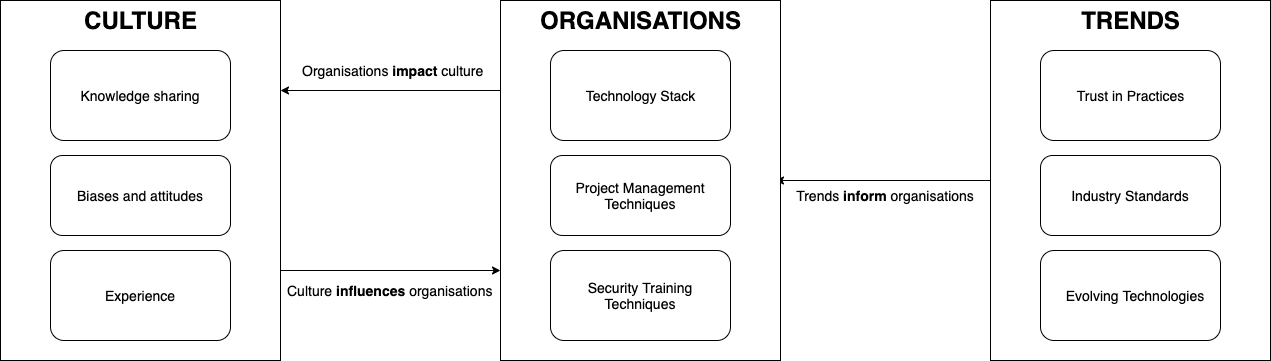
\includegraphics[width=17cm]{figures/fig2.png}
\centering
\caption{The Theory of Influences on Security Practices}
\centering
\end{figure}

\par
Culture referenced knowledge sharing, biases and attitudes. The category is a combination of the culture we see in groups of individuals, and the term culture refers to the customs that programmers have in order to maintain security. Knowledge sharing was internal team communications between members. Biases and attitudes were existing thoughts and feelings on how they implement and learn about security. Experience was the number of the number of threats programmers had been exposed to. 
\newline
\par
Organisations included the attributes, technology stack, project management techniques and security training techniques. The technology stack was the programming languages, libraries, frameworks and tools that were in use by the participants. Project management techniques were management structures enforced within the organisation; whether this is Waterfall, Agile or DevOps. The security training techniques were the avenues of educational support provided by different organisations.  
\newline
\par
Trends specified that trust in practices, industry standards and evolving technologies were due to the influences of industry trends on a programmer. Trust in practices was the lack of checking open-source technology; the industry standard was changing policies, compliance and best-practice standards. Evolving technologies referenced the ever-changing adoption of new technology to business streams.
\newline
\par 
The emergent theory has been evaluated Glaser's criteria of fit, work, relevance and modifiability. It provides a theory which is thoroughly explained, has drawn codes from newly gathered information, is relevant to the topic and can adapt long-term. The theory has also been evaluated against three works of literature. Overall, the findings of this research can provide a more robust educational programme in the workplace and allow for companies to reevaluate how they respond to trends, how they structure their organisations and what they do to improve their culture.

\section{Implications for Practice}

The emergent theory defined three main categories and a further nine attributes for the influences on security practices. By understanding how they each relate to each other, organisations can implement changes in how they react to trends and how they deal with and motivate changes in culture. 
\newline
\par
In New Zealand, there have been some small changes with a participant \textit{[P7] } having completed a Hackathon when joining the organisation, but this change needs to be long-lasting, and there should be constant practical ways to learn about secure programming much like the once a month opportunities that \textit{[P14]} has. This will reinforce security a part of the culture of programmers way-of-working. 
 \newline
 \par
 There needs to be reform in how security is taught in organisations. There should be more support for programmers in terms of technical education within organisations instead of just the general policy and practices that all employees get. Technical education will be best done with frequent, optional internal Hackathons. \textit{[P14]}, described giving cases related to the nature of the organisations work, and this provided a mock scenario which can build up the experiences of employees in a safe environment without any consequences. It also introduces programmers to a diverse technology-stack, and as organisations continue to adapt to the popular trends in the industry, employees need to experience more languages, tools, frameworks, libraries. The range and growth of the experiences which are provided by the organisation in-turn increase the ability for employees to deal with security issues and become more open to changes in the normal day-to-day.  
 \newline
 \par
 Employees will benefit if cross-functional teams are used within organisations. When this trend rises to include security-focused team-members, it will make implementing security in software easier for programmers. Security is a growing field so as the current issues with a lack of money and skillset will reduce as it starts to hold more gain \cite{grow}. 
 

\section{Limitations and Future Work} 

\par There were some limitations in regard to the data collection. While not significant, there was a gender imbalance in the participants. One third were female while the rest male. As women are underrepresented in STEM (Science, Technology, Engineering and Mathematics) fields \cite{wit}, it can be argued that this is indicative of the actual population. However, as women in this industry typically have different experiences to the majority, it would have been interesting to have more varying data to draw codes from \cite{wit}. 
\newline
\par
Another difficulty that limited the theory when data collecting was the refusal to answer questions. Due to non-disclosure agreements, for some participants, this was so strict that they could not answer questions such as, "what language do you use to program with at work?". This made it challenging to draw appropriate conclusions during the middle of this study. This could have also introduced slight biases in the collection as observational inferences were made based on the non-responses. 
\newline
\par
While it was interesting to obtain a diverse range of experiences within the sample group of participants, for future work, the investigation would benefit from reducing this scope. By choosing one type of role, one sector or similar years of experience, the theory would have had some more pointers to technical influences. This would have resulted in critical traits for a programmer to improve upon in their security education directly. It could also provide more insights as to why specific programmers seem to find security a hindrance and how to change this. A suggestion would be to focus on cloud engineers as they were the only ones in this study that indicated that languages and libraries change based on security needs. If future studies could focus on organisational differences, it would be interesting as smaller companies had laxer security controls and support when programming compared to the more prominent companies. Smaller organisations, however, seemed to be more willing and open to change than those in an established organisation.
\newline
\par 
A separate study on internal Hackathons could be undertaken. As it is a relatively new concept in New Zealand and there generally is a paucity of research worldwide, so it would be interesting to combine the two; Corporate Hackathons in New Zealand. Specifically focusing on the differences between less experienced people and more experienced people in terms of work experience and the impacts before, during and after a Hackathon using the Phenomenology methodology could form a strong understanding of the effects on a varying group's experiences due to such an event. It can be used to market the idea of having regular internal Hackathons within organisations in New Zealand. 




%%%%%%%%%%%%%%%%%%%%%%%%%%%%%%%%%%%%%%%%%%%%%%%%%%%%%%%

\backmatter

%%%%%%%%%%%%%%%%%%%%%%%%%%%%%%%%%%%%%%%%%%%%%%%%%%%%%%%


\bibliographystyle{ieeetr}
\bibliography{7-references}
\bibliographystyle{ieeetr}

% appendix
\appendix
\chapter{Human Ethics Application}
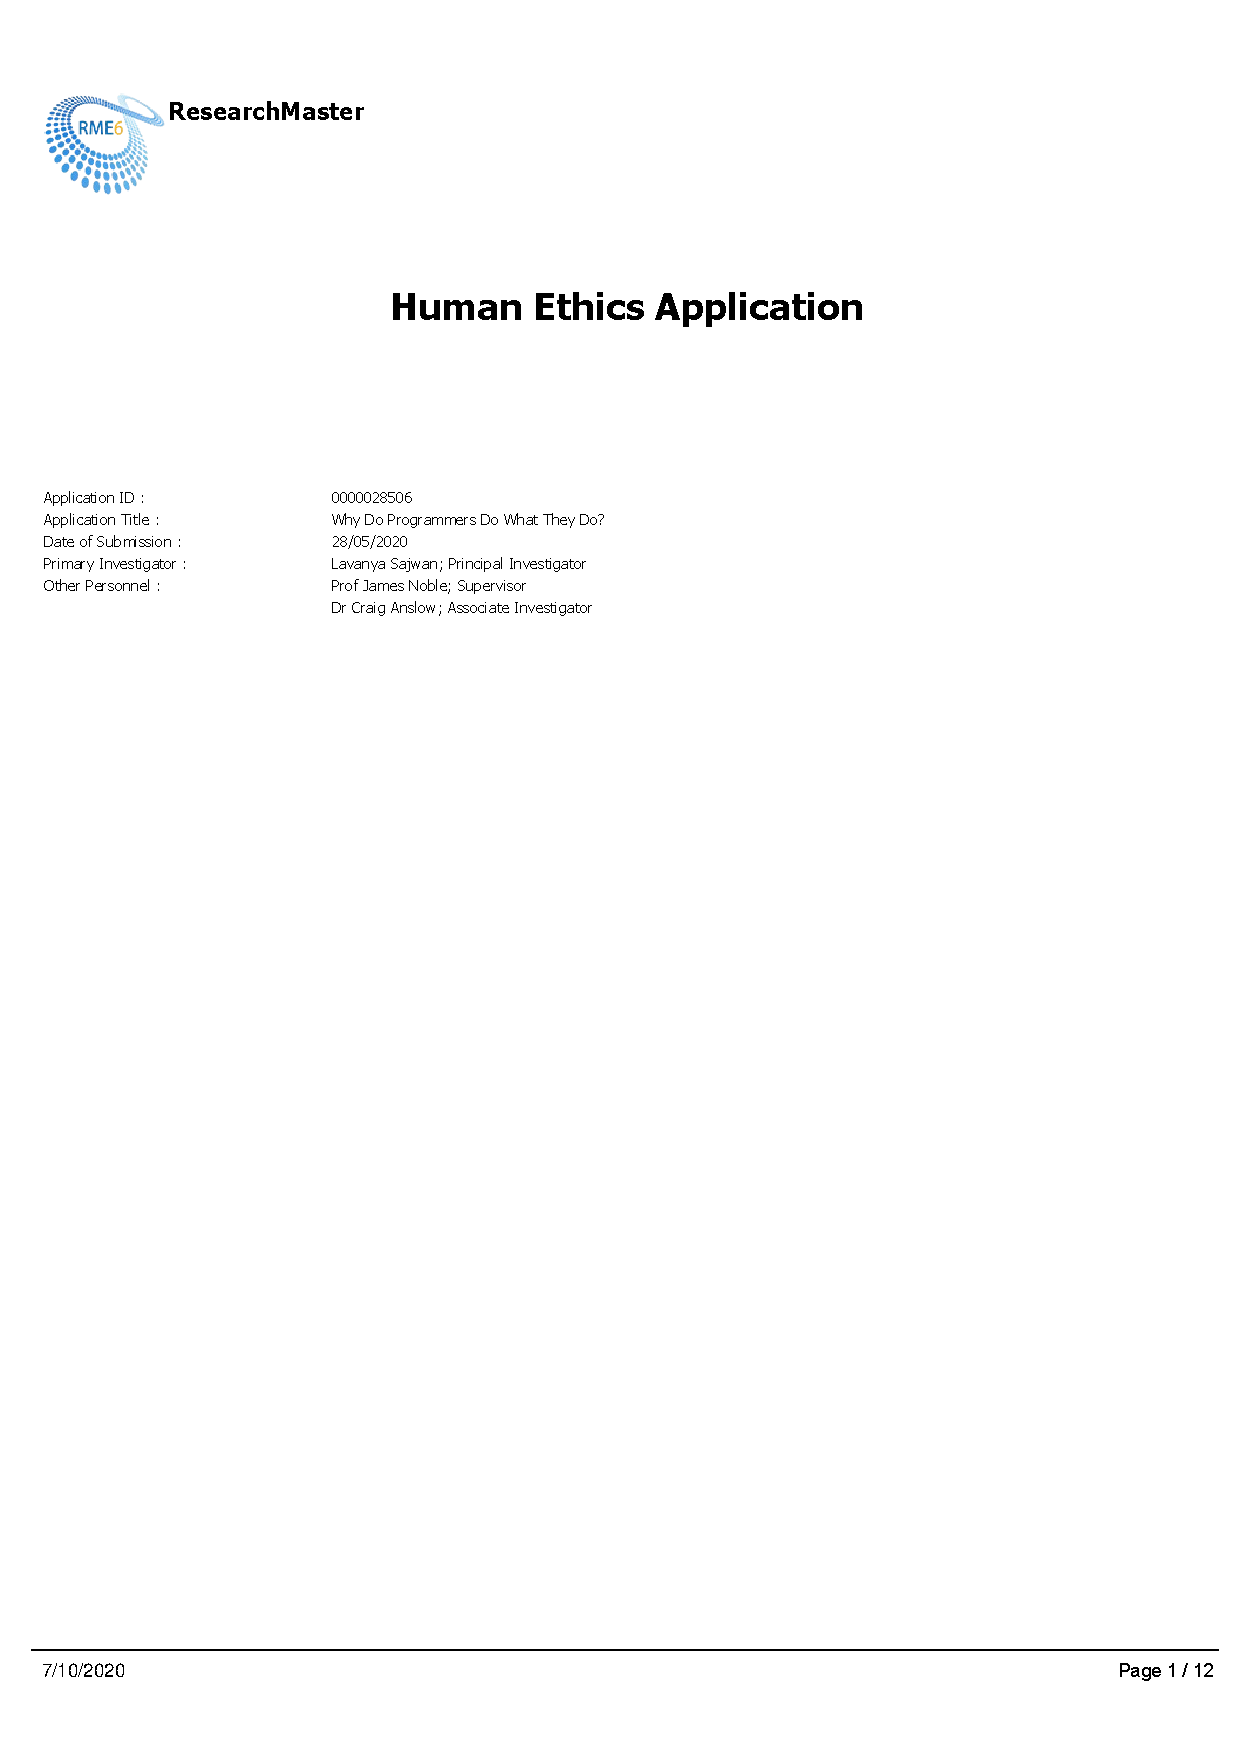
\includegraphics[height=0.8\textheight]{appendix/humanethics.pdf}
\includepdf[pagecommand={\thispagestyle{plain}}, pages={2-last},scale=0.8]{appendix/humanethics.pdf}





\chapter{Participant Information Sheet}
\includegraphics[height=0.8\textheight]{\string"Participant_Information_Sheet".pdf}

\includepdf[pagecommand={\thispagestyle{plain}}, pages={2-last},scale=0.8]{Participant_Information_Sheet.pdf}


\chapter{Participant Consent Form}

\includegraphics[height=0.8\textheight]{appendix/consent.pdf}

\includepdf[pagecommand={\thispagestyle{plain}}, pages={2-last},scale=0.8]{appendix/consent.pdf}


\chapter{Interview Template}
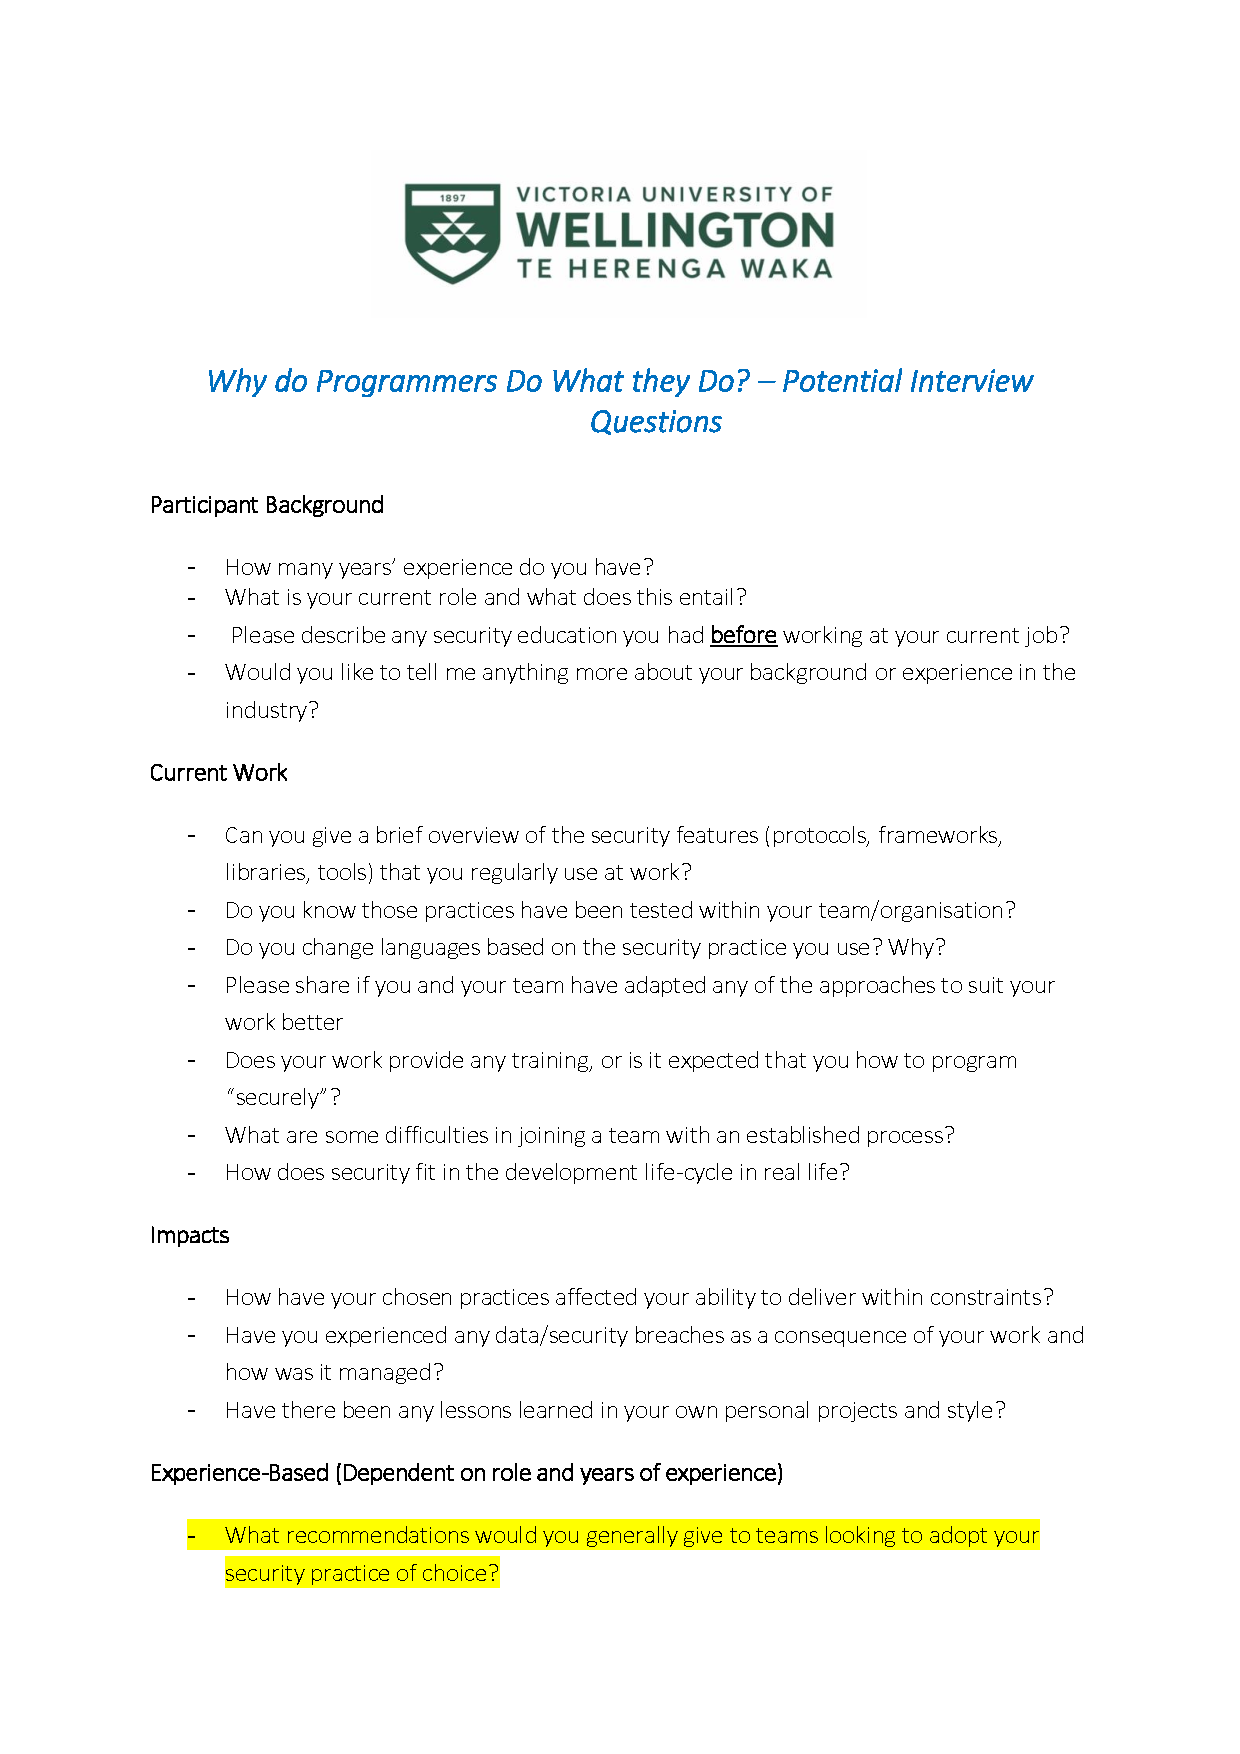
\includegraphics[height=0.8\textheight]{appendix/questions.pdf}
\includepdf[pagecommand={\thispagestyle{plain}}, pages={2-last},scale=0.8]{appendix/questions.pdf}


\chapter{Recruitment Post}

\includegraphics[height=0.8\textheight]{appendix/post.pdf}
\chapter{Recruitment Webpage}
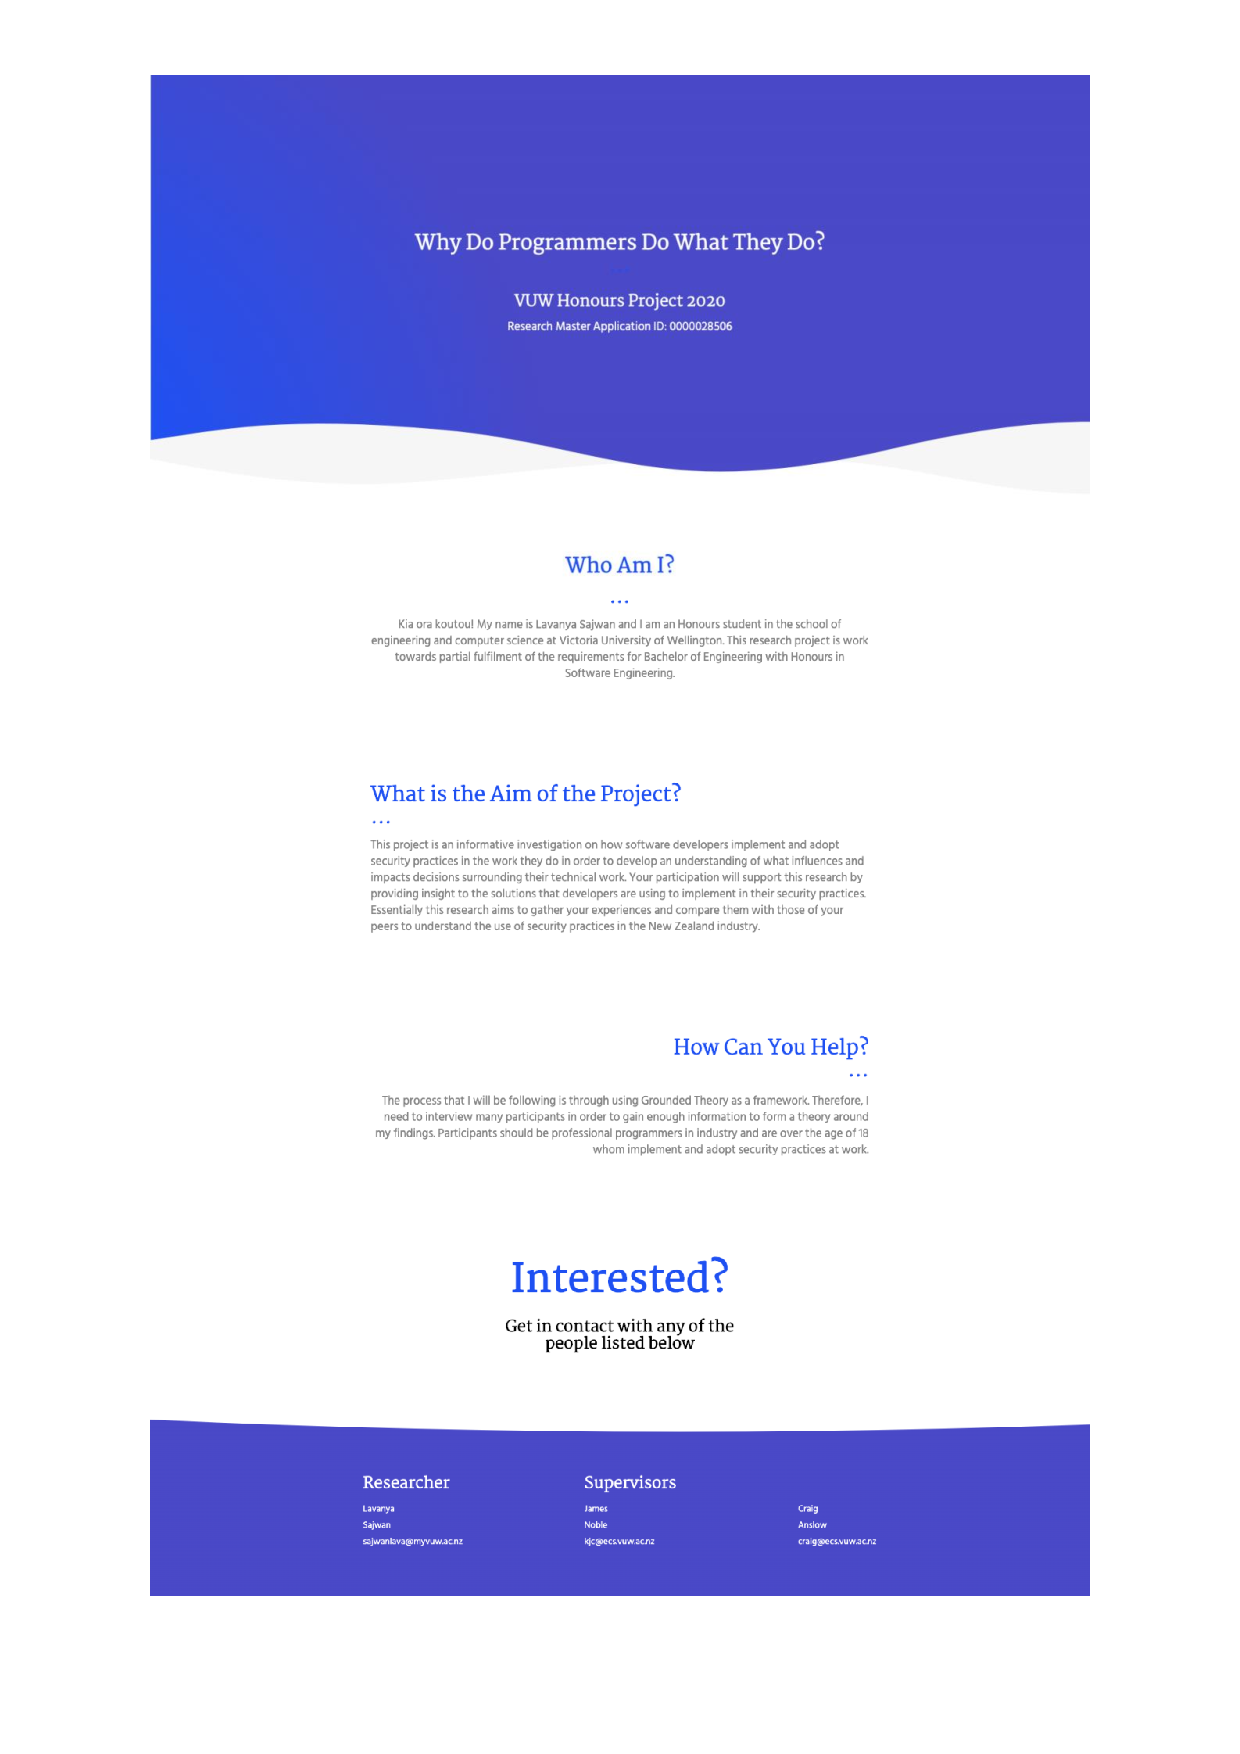
\includegraphics[width=\textwidth]{appendix/webpage.pdf}



\end{document}
